\def\linkdethi{} %Đường link cần dẫn tới
\anmaQR
%%%%%%%%%%%%%%%%%%%%%%%%
\def\toanlop{12}
\def\thoigian{90}
\def\namhoc{2025 - 2026}
\begin{dethi}
	{Bộ GD\&ĐT}
	{VTED ft KING EDU}
	{TDMZD01}
	{Đề thi thử THPTQG 2026}
\end{dethi}

\caulc
\Opensolutionfile{ans}[ans/ansTN-Dung]
%%%=============EX_1=============%%%
\begin{ex}%[2D4N1-4]%[TDMZD01]%[Trần Văn Thiện]
	Họ nguyên hàm của hàm số $f(x)=3^{x+1}$ là
	\choice
	{\True $\dfrac{3^{x+1}}{\ln 3}+C$}
	{$\dfrac{3^{x}}{\ln 3}+C$}
	{$\dfrac{3^{x+2}}{x+2}+C$}
	{$3^{x+1}+C$}
	\loigiai{
		Ta có $\displaystyle\int 3^{x+1}\,\mathrm{d}x 
		=\displaystyle\int 3\cdot 3^x \,\mathrm{d}x 
		=3\cdot\dfrac{3^x}{\ln 3}+C 
		=\dfrac{3^{x+1}}{\ln 3}+C$.
	}
\end{ex}
%%%=============================%%%

%%%=============EX_2=============%%%
\begin{ex}%[2D4N3-1]%[TDMZD01]%[Phạm Hải Dương]
	Diện tích hình phẳng giới hạn bởi các đường $y=f(x)$, $y=g(x)$, $x=a$, $x=b$ ($a<b$) được tính theo công thức
	\choice
	{$S=\pi\displaystyle\int\limits_{a}^{b}\left|f(x)-g(x)\right|\,\mathrm{d}x$}
	{\True $S=\displaystyle\int\limits_{a}^{b}\left|f(x)-g(x)\right|\,\mathrm{d}x$}
	{$S=\displaystyle\int\limits_{a}^{b}\left[f(x)-g(x)\right]\,\mathrm{d}x$}
	{$S=\displaystyle\int\limits_{a}^{b}\left|f(x)\right|\,\mathrm{d}x-\displaystyle\int\limits_{a}^{b}\left|g(x)\right|\,\mathrm{d}x$}
	\loigiai{
		Công thức tính diện tích hình phẳng giới hạn bởi các đường $y=f(x)$, $y=g(x)$, $x=a$, $x=b$ ($a<b$) được tính theo công thức $S=\displaystyle\int\limits_{a}^{b}\left|f(x)-g(x)\right|\,\mathrm{d}x$.
	}
\end{ex}
%%%=============================%%%

%%%=============EX_3=============%%%
\begin{ex}%[2D3H2-2]%[TDMZD01]%[Văn Minh Thoại]
	Cho hai mẫu số liệu $M_1$, $M_2$ với bảng tần số ghép nhóm như sau
	\begin{center}
		\begin{tabular}{ll}
			Nhóm $M_1$&
			\begin{tabular}{|c|c|c|c|c|c|c|}
				\hline
				Nhóm & $[5;7)$ & $[7;9)$ & $[9;11)$ & $[11;13)$ & $[13;15)$ & $[15;17)$ \\
				\hline
				Tần số & $3$ & $5$ & $6$ & $4$ & $6$ & $9$ \\
				\hline
			\end{tabular}\\
			&\\
			Nhóm $M_2$&
			\begin{tabular}{|c|c|c|c|c|c|c|}
				\hline
				Nhóm & $[5;7)$ & $[7;9)$ & $[9;11)$ & $[11;13)$ & $[13;15)$ & $[15;17)$ \\
				\hline
				Tần số & $6$ & $10$ & $12$ & $8$ & $12$ & $18$ \\
				\hline
			\end{tabular}
		\end{tabular}
	\end{center}
	Hãy so sánh độ lệch chuẩn $s_1$, $s_2$ của hai mẫu số liệu $M_1$, $M_2$.
	\choice
	{$s_1<s_2$}
	{\True $s_1=s_2$}
	{$s_1=2s_2$}
	{$s_1=3s_2$}
	\loigiai{
		Xét mẫu số liệu $M_1$, ta được
		\begin{center}
			\begin{tabular}{ll}
				Nhóm $M_1$&
				\begin{tabular}{|c|c|c|c|c|c|c|}
					\hline
					Nhóm & $[5;7)$ & $[7;9)$ & $[9;11)$ & $[11;13)$ & $[13;15)$ & $[15;17)$ \\
					\hline
					Giá trị đại diện & $6$ & $8$ & $10$ & $12$ & $14$ & $16$ \\
					\hline
					Tần số & $3$ & $5$ & $6$ & $4$ & $6$ & $9$ \\
					\hline
				\end{tabular}
			\end{tabular}
		\end{center}
		\begin{itemize}
			\item Cỡ mẫu là $n_1=3+5+6+4+6+9=33$.
			\item Số trung bình là
			\[\overline{x}_1 = \dfrac{3 \cdot 6 + 5 \cdot 8 + 6 \cdot 10 + 4 \cdot 12 + 6 \cdot 14 + 9 \cdot 16}{33} = \dfrac{394}{33}.\]
			\item Phương sai là
			\[s_1^2 = \dfrac{1}{33}\left(3 \cdot 6^2 + 5 \cdot 8^2 + 6 \cdot 10^2 + 4 \cdot 12^2 + 6 \cdot 14^2 + 9 \cdot 16^2\right)- \left(\dfrac{394}{33}\right)^2 \approx 11{,}51.\]
			\item Độ lệch chuẩn là $s_1=\sqrt{s_1^2}\approx 3{,}39$.
		\end{itemize}
		Xét mẫu số liệu $M_2$, ta được
		\begin{center}
			\begin{tabular}{ll}
				Nhóm $M_2$&
				\begin{tabular}{|c|c|c|c|c|c|c|}
					\hline
					Nhóm & $[5;7)$ & $[7;9)$ & $[9;11)$ & $[11;13)$ & $[13;15)$ & $[15;17)$ \\
					\hline
					Giá trị đại diện & $6$ & $8$ & $10$ & $12$ & $14$ & $16$ \\
					\hline
					Tần số & $6$ & $10$ & $12$ & $8$ & $12$ & $18$ \\
					\hline
				\end{tabular}
			\end{tabular}
		\end{center}
		\begin{itemize}
			\item Cỡ mẫu là $n_2=6+10+12+8+12+18=66$.
			\item Số trung bình là
			\[\overline{x}_2 = \dfrac{6 \cdot 6 + 10 \cdot 8 + 12 \cdot 10 + 8 \cdot 12 + 12 \cdot 14 + 18 \cdot 16}{66} = \dfrac{788}{66} = \dfrac{394}{33} .\]
			\item Phương sai là
			\[s_2^2 = \dfrac{1}{66} \left(6 \cdot 6^2 + 10 \cdot 8^2 + 12 \cdot 10^2 + 8 \cdot 12^2 + 12 \cdot 14^2 + 18 \cdot 16^2\right)- \left(\dfrac{394}{33}\right)^2 \approx 11{,}51.\]
			\item Độ lệch chuẩn là $s_2=\sqrt{s_2^2}\approx 3{,}39$.
		\end{itemize}
		Vậy $s_1=s_2$.
	}
\end{ex}
%%%=============================%%%

%%%=============EX_4=============%%%
\begin{ex}%[2D1N2-2]%[TDMZD01]%[Lê Phúc]
	\immini[thm]{Cho hàm số $y=ax^3+bx^2+cx+d$ ($a\neq 0$) có đồ thị như hình vẽ.
		Giá trị cực đại của hàm số là
		\choice
		{$1$}
		{\True $2$}
		{$(1;2)$}
		{$-1$}
	}
	{
		\begin{tikzpicture}[line cap=butt,line join=miter,>=stealth]
			\draw[->] (-3,0)--(4,0)
			node[shift={(-100:7pt)},font=\normalsize]{$x$};
			\draw[->] (0,-2)--(0,3)
			node[shift={(180:7pt)},font=\normalsize]{$y$};
			\draw (5pt,0) |- (0,5pt)
			(0,0) node[shift={(225:9pt)},font=\normalsize]{$O$};
			\foreach \x in {2}{
				\draw (\x,1.5pt)--(\x,-1.5pt) node[font=\scriptsize,shift={(90:8pt)}]{\x};
			}
			\foreach \x in {-1}{
				\draw (\x,1.5pt)--(\x,-1.5pt) node[font=\scriptsize,shift={(-90:8pt)}]{\x};
			}
			\foreach \y in {2}{
				\draw (1.5pt,\y)--(-1.5pt,\y) node[font=\scriptsize,shift={(0:8pt)}]{\y};
			}
			\foreach \y in {-1}{
				\draw (1.5pt,\y)--(-1.5pt,\y) node[font=\scriptsize,shift={(180:8pt)}]{\y};
			}
			\draw[dashed] (0,2)--(-1,2) (2,0)--(2,-1)--(0,-1) (-1,0)--(-1,2);
			\foreach \p in {(0,0), (0,-1), (-1,0) ,(-1,2), (2,-1), (0,11/9), (0.825,0)}{
				\fill \p circle (1pt);
			}
			\tikzset{declare function={f (\x)=2/9*((\x)^3)+-1/3*((\x)^2)+-4/3*(\x)+11/9;}}
			\begin{scope}
				\draw[samples=100] plot[domain=-2.5:3.5] (\x,{f (\x)});
			\end{scope}
		\end{tikzpicture}
	}
	\loigiai{
		Dựa vào đồ thị hàm số ta thấy giá trị cực đại của hàm số là $y_{\text{CĐ}}=2$.
	}
\end{ex}
%%%=============================%%%

%%%=============EX_5=============%%%
\begin{ex}%[2H5N2-3]%[TDMZD01]%[Vũ Hồng Toàn]
	Trong không gian $Oxyz$, phương trình tham số của trục $Ox$ là
	\choice
	{$\heva{&x=0\\&y=t\\&z=0}\,(t\in\mathbb{R})$}
	{$\heva{&x=0\\&y=t\\&z=t}\,(t\in\mathbb{R})$}
	{$\heva{&x=0\\&y=0\\&z=t}\,(t\in\mathbb{R})$}
	{\True $\heva{&x=t\\&y=0\\&z=0}\,(t\in\mathbb{R})$}
	\loigiai{
		Trục $Ox$ đi qua gốc tọa độ $O(0;0;0)$ và có vectơ chỉ phương $\overrightarrow{i}=(1;0;0)$.\\
		Phương trình tham số của trục $Ox$ là $\heva{&x=t\\&y=0\\&z=0}\,(t\in\mathbb{R})$.
	}
\end{ex}
%%%=============================%%%

%%%=============EX_6=============%%%
\begin{ex}%[1D6N4-2]%[TDMZD01]%[Chu Hà]
	Tập nghiệm của bất phương trình $\log(x-3)<1$ là
	\choice
	{$\left\lbrace 3;13\right\rbrace$}
	{$\left(-\infty;13\right)$}
	{$\left(13;+\infty\right)$}
	{\True $\left(3;13\right)$}
	\loigiai{
		Điều kiện xác định $x-3 > 0 \Leftrightarrow x > 3$.\\
		Ta có
		\allowdisplaybreaks
		\begin{eqnarray*}
			&&\log(x-3) < 1\\
			&\Leftrightarrow& x-3 < 10^1\,\,(\text{do cơ số thập phân $10>1$})\\
			&\Leftrightarrow& x-3 < 10\\
			&\Leftrightarrow& x < 13.
		\end{eqnarray*}
		Kết hợp điều kiện xác định $x>3$ ta được $3 < x < 13$.\\
		Vậy tập nghiệm của bất phương trình $\log(x-3)<1$ là $\left(3;13\right)$.
	}
\end{ex}
%%%=============================%%%

%%%=============EX_7=============%%%
\begin{ex}%[2H5N1-2]%[TDMZD01]%[Nguyễn Sơn Thành]
	Trong không gian $Oxyz$, cho phương trình mặt phẳng $(\alpha) \colon 2x+2y-3=0$. Hỏi vectơ nào dưới đây là vectơ pháp tuyến của $\left(\alpha\right)$?
	\choice
	{$\overrightarrow{n}_1=\left(2;2;-3\right)$}
	{$\overrightarrow{n}_2=\left(2;2;-1\right)$}
	{\True $\overrightarrow{n}_3=\left(2;2;0\right)$}
	{$\overrightarrow{n}_4=\left(2;2;3\right)$}
	\loigiai{
		Mặt phẳng $(\alpha) \colon 2x + 2y - 3 = 0$ có vectơ pháp tuyến là $\left(2; 2; 0\right)$.}
\end{ex}
%%%=============================%%%

%%%=============EX_8=============%%%
\begin{ex}%[1H8H4-2]%[TDMZD01]%[Đỗ Đường Hiếu]
	Cho hình chóp $S.ABCD$ có đáy $ABCD$ là hình chữ nhật, $SA \perp (ABCD)$. Trong các mặt phẳng cho dưới đây, mặt phẳng \textbf{không} vuông góc với mặt phẳng $(ABCD)$ là
	\choice
	{$(SAC)$}
	{$(SAD)$}
	{$(SAB)$}
	{\True $(SBC)$}
	\loigiai{
		\immini{
			Vì $SA \perp (ABCD)$ nên mọi mặt phẳng chứa $SA$ đều vuông góc với $(ABCD)$.\\
			Các mặt phẳng $(SAC)$, $(SAD)$, $(SAB)$ đều chứa $SA$ nên các mặt phẳng $(SAC)$, $(SAD)$, $(SAB)$ đều vuông góc với $(ABCD)$.\\
			Ta có $\heva{&BC\perp SA\\&BC\perp AB}\Rightarrow BC\perp (SAB)\Rightarrow BC\perp SB$.}
		{
			\begin{tikzpicture}[declare function={gocx=90; goc=-150; a=3.2; b=a/2; h=3;}]
				\path (0,0) coordinate (A)--+(gocx:h) coordinate (S)
				(a,0) coordinate (D)
				(goc:b) coordinate (B)
				+(a,0) coordinate (C);
				\foreach \x/\y/\z in {S/A/D,S/A/B}{
					\path (\y) pic[draw,angle radius=4pt]{right angle = \x--\y--\z};
				}
				\draw[dashed] (S)--(A) (B)--(A)--(D) (A)--(C);
				\draw (S)--(B)--(C)--(S)--(D)--(C)--cycle;
				\foreach \x/\goc in {S/90,A/-90,D/0,C/-60,B/-180}
				\fill (\x) node[shift={(\goc:7pt)},font=\scriptsize]{$\x$} circle (1pt);
			\end{tikzpicture}
		}
		\noindent Giả sử mặt phẳng $(SBC)\perp (ABCD)$, khi đó $BC$ là giao tuyến của hai mặt phẳng $(SBC)$ và $(ABCD)$, $SB\perp BC$ nên suy ra $SB\perp (ABCD)$.\\
		Nếu thế thì qua $S$ có hai đường thẳng $SA$, $SB$ cùng vuông góc với mặt phẳng $(ABCD)$, điều này không thể xảy ra.\\
		Vậy mặt phẳng $(SBC)$ không vuông góc với mặt phẳng $(ABCD)$.
	}
\end{ex}
%%%=============================%%%

%%%=============EX_9=============%%%
\begin{ex}%[1D6N4-2]%[TDMZD01]%[Huỳnh Quốc Đạt]
	Nghiệm của phương trình $2^x=256$ là
	\choice
	{\True $x=8$}
	{$x=9$}
	{$x=4$}
	{$x=128$}
	\loigiai{
		Ta có
		\allowdisplaybreaks
		\begin{eqnarray*}
			&&2^x = 256 \\
			&\Leftrightarrow& 2^x=2^8\\
			&\Leftrightarrow& x=8.
		\end{eqnarray*}
		Vậy nghiệm của phương trình $2^x=256$ là $x=8$.
	}
\end{ex}
%%%=============================%%%

%%%=============EX_10=============%%%
\begin{ex}%[1D2H3-4]%[TDMZD01]%[Dương Công Tạo]
	Cho cấp số nhân $\left(u_n\right)$ có $u_1=1$, $u_2=3$. Số hạng thứ ba của $\left(u_n\right)$ bằng
	\choice
	{\True $9$}
	{$27$}
	{$5$}
	{$6$}
	\loigiai{
		Công bội của cấp số nhân $\left(u_n\right)$ là $q = \dfrac{u_2}{u_1} = 3$.\\
		Khi đó, số hạng thứ ba của $\left(u_n\right)$ là $u_3 = u_1 \cdot q^2 = 1 \cdot 3^2 = 9$.
	}
\end{ex}
%%%=============================%%%

%%%=============EX_11=============%%%
\begin{ex}%[2H2N1-2]%[TDMZD01]%[Nguyễn Tấn Linh]
	\immini[thm]
	{
		Cho hình chóp đều $S.ABCD$ có tâm của đáy là $O$. Hỏi phát biểu nào dưới đây \textbf{sai}?
		\choice
		{\True $\overrightarrow{SA}-\overrightarrow{SC}=2\overrightarrow{SO}$}
		{$\overrightarrow{SB}+\overrightarrow{SD}=2\overrightarrow{SO}$}
		{$\overrightarrow{SB}-\overrightarrow{SD}=\overrightarrow{DB}$}
		{$\overrightarrow{SA}+\overrightarrow{SB}+\overrightarrow{SC}+\overrightarrow{SD}=4\overrightarrow{SO}$}
	}
	{
		\begin{tikzpicture}[font=\scriptsize]
			\tikzset{declare function={a=3; b=2; h=3.2;}}
			\path (0,0) coordinate (A)
			(a,0) coordinate (D)
			(-145:b) coordinate (B)
			($(B)+(D)$) coordinate (C)
			($(A)!0.5!(C)$) coordinate (O)
			($(O)+(0,h)$) coordinate (S);
			\path pic[draw,angle radius=4pt]{right angle=A--O--S};
			\path pic[draw,angle radius=4pt]{right angle=D--O--S};
			\draw[dashed] (B)--(A)--(D)--cycle (C)--(A)--(S)--(O);
			\draw (S)--(B)--(C)--(D)--cycle (S)--(C);
			\foreach \t/\g in {A/150,B/180,C/-30,D/0,S/90,O/-90}{
				\fill (\t) circle (1pt) node[shift={(\g:7pt)},font=\scriptsize]{$\t$};
			}
		\end{tikzpicture}
	}
	\loigiai{
		Vì $ABCD$ là đáy của hình chóp đều tâm $O$ nên $O$ là trung điểm của $AC$ và $BD$.\\
		Ta có các khẳng định sau
		\begin{itemize}
			\item Theo quy tắc trung điểm $\overrightarrow{SB}+\overrightarrow{SD}=2\overrightarrow{SO}$.
			\item $\overrightarrow{SA}+\overrightarrow{SB}+\overrightarrow{SC}+\overrightarrow{SD}=\left(\overrightarrow{SA}+\overrightarrow{SC}\right)+\left(\overrightarrow{SB}+\overrightarrow{SD}\right)=2\overrightarrow{SO}+2\overrightarrow{SO}=4\overrightarrow{SO}$.
			\item $\overrightarrow{SB}-\overrightarrow{SD}=\overrightarrow{DB}$.
		\end{itemize}
		Do đó  $\overrightarrow{SA}-\overrightarrow{SC}=\overrightarrow{CA}\neq 2\overrightarrow{SO}$.
	}
\end{ex}
%%%=============================%%%

%%%=============EX_12=============%%%
\begin{ex}%[2D1N2-1]%[TDMZD01]%[Duong Xuan Loi]
	Hàm số $y=x^3-3x^2-1$
	\choice
	{\True đạt cực đại tại $x=0$}
	{đạt cực tiểu tại $x=1$}
	{đồng biến trên $\mathbb{R}$}
	{nghịch biến trên khoảng $(-1;1)$}
	\loigiai{
		Ta có $y=x^3-3x^2-1$.\\
		Suy ra $y'= 3x^2-6x$.\\
		Khi đó $y'=0 \Leftrightarrow \hoac{&x=0\\&x=2.}$\\
		Bảng biến thiên
		\begin{center}
			\begin{tikzpicture}[font=\normalsize,t style/.style={style=solid}]
				\tkzTabInit[nocadre=false, lgt=1.2, espcl=2.5, deltacl=0.5]
				{$x$/0.75, $y'$/0.75, $y$/3}
				{$-\infty$, $0$, $2$, $+\infty$}
				\tkzTabLine{ , +, 0, -, 0, +}
				\path
				($(N13)!0.1!(N12)$) node (A1){$ -\infty $}
				($(N23)!0.7!(N22)$) node (A2){$ -1 $}
				($(N33)!0.3!(N32)$) node (A3){$ -5 $}
				($(N43)!0.8!(N42)$) node (A4){$ +\infty $};
				\foreach \x/\y in {A1/A2, A2/A3, A3/A4}{
					\draw[-stealth] (\x)--(\y);
				}
			\end{tikzpicture}
		\end{center}
		Dựa vào bảng biến thiên ta thấy
		\begin{itemize}
			\item Hàm số đạt cực đại tại $x=0$.
			\item Hàm số đạt cực tiểu tại $x=2$.
			\item Hàm số nghịch biến trên khoảng $(0;2)$.
			\item Hàm số đồng biến trên khoảng $(-\infty;0)$ và $(2;+\infty)$.
		\end{itemize}
	}
\end{ex}
%%%=============================%%%
\Closesolutionfile{ans}

\cauds
\Opensolutionfile{ans}[ans/ansTN-DungSai]
%%%=============EX_13=============%%%
\begin{ex}%[2D1V5-7]%[TDMZD01]%[Hmh]
	Cho hàm số $y=f(x)=\dfrac{3x+1}{x-1}$ có đồ thị $(C)$.
	\choiceTF[t]
	{\True Hàm số $f(x)$ không có cực trị}
	{\True Tâm đối xứng của $(C)$ là $I(1;3)$}
	{\True $(C)$ có tất cả $6$ điểm mà hoành độ và tung độ của nó là các số nguyên}
	{\True Số đường parabol dạng $y=ax^2+bx+c$ ($a$, $b$, $c \in \mathbb{R}$) cắt $(C)$ tại ba điểm phân biệt có tọa độ nguyên là $20$}
	\loigiai{
		\begin{itemchoice}
			\itemch Tập xác định $\mathscr{D}=\mathbb{R} \setminus \{1\}$.\\
			Ta có $y'=\dfrac{3(x-1)-(3x+1)}{(x-1)^2}
			=\dfrac{3x-3-3x-1}{(x-1)^2}
			= \dfrac{-4}{(x-1)^2} < 0$, $\forall x \neq 1$.\\
			Vì đạo hàm luôn âm và không có nghiệm nên hàm số không có cực trị.
			\itemch Đồ thị hàm số có tiệm cận đứng $x=1$ và tiệm cận ngang $y=3$.\\
			Giao điểm hai đường tiệm cận là tâm đối xứng của đồ thị.\\ Suy ra $I(1;3)$.
			\itemch Ta có $y = \dfrac{3x+1}{x-1} = \dfrac{3(x-1)+4}{x-1} = 3 + \dfrac{4}{x-1}$.\\
			Để điểm thuộc $(C)$ có tọa độ nguyên thì $x$ và $y$ phải là số nguyên, suy ra $(x-1)$ phải là ước của $4$.\\
			Các ước của $4$ là $\{-4; -2; -1; 1; 2; 4\}$.\\
			Ta có bảng giá trị
			\begin{center}
				\begin{tabular}{|c|c|c|c|c|c|c|}
					\hline
					$x-1$ & $-4$ & $-2$ & $-1$ & $1$ & $2$ & $4$ \\
					\hline
					$x$ & $-3$ & $-1$ & $0$ & $2$ & $3$ & $5$ \\
					\hline
					$y$ & $2$ & $1$ & $-1$ & $7$ & $5$ & $4$ \\
					\hline
				\end{tabular}
			\end{center}
			Vậy có $6$ điểm có tọa độ nguyên thuộc đồ thị $(C)$.
			\itemch Gọi tập hợp các điểm có tọa độ nguyên trên $(C)$ là $S$.\\ Theo câu c, số phần tử của $S$ là $6$.\\
			Phương trình hoành độ giao điểm của một đường thẳng bất kỳ $y=mx+n$ và đồ thị $(C)$ là
			\[mx+n = \dfrac{3x+1}{x-1} \Leftrightarrow mx^2 + (n-m-3)x - n - 1 = 0 \quad (*).\]
			Phương trình $(*)$ là phương trình bậc hai (hoặc bậc nhất) nên có tối đa $2$ nghiệm.\\ Do đó, một đường thẳng bất kỳ cắt $(C)$ tại tối đa $2$ điểm.\\ Suy ra không có $3$ điểm nào thuộc $(C)$ thẳng hàng.\\
			Một đường parabol $y=ax^2+bx+c$ được xác định duy nhất bởi $3$ điểm không thẳng hàng.\\
			Do đó, số đường parabol đi qua $3$ điểm phân biệt trong tập $S$ chính là số tổ hợp chập $3$ của $6$ phần tử
			\[ \mathrm{C}_6^3 = \dfrac{6!}{3!(6-3)!} = 20 \text{ (đường)}. \]
		\end{itemchoice}
	}
\end{ex}
%%%=============================%%%

%%%=============EX_14=============%%%
\begin{ex}[Đề chính thức THPTQG 2025]%[2D4V2-6]%[TDMZD01]%[Lê Minh]
	Đối với ngành nuôi trồng thủy sản, việc kiểm soát lượng thuốc tồn dư trong nước là một nhiệm vụ quan trọng nhằm đáp ứng các tiêu chuẩn an toàn về môi trường. Khi nghiên cứu một loại thuốc trị bệnh trong nuôi trồng thủy sản, người ta sử dụng thuốc đó một lần và theo dõi nồng độ thuốc tồn dư trong nước kể từ lúc sử dụng thuốc. Kết quả cho thấy nồng độ thuốc $y(t)$ (đơn vị: mg/lít) tồn dư trong nước tại thời điểm $t$ ngày ($t\geq 0$) kể từ lúc sử dụng thuốc, thỏa mãn $y(t) > 0$ và $y'(t)=k\cdot y(t)$ ($t\geq 0$), trong đó $k$ là hằng số khác không. Đo nồng độ thuốc tồn dư trong nước tại thời điểm $t=6$ (ngày); $t=12$ (ngày) nhận được kết quả lần lượt là $2$ mg/lít; $1$ mg/lít. Cho biết $y(t)=\mathrm{e}^{g(t)}$ ($t\geq 0$).
	\choiceTF[t]
	{\True $g(t)=kt+C$ ($t\geq 0$) với $C$ là một hằng số xác định}
	{$k=\dfrac{\ln 2}{6}$}
	{\True $C=2\ln 2$}
	{Nồng độ thuốc tồn dư trong nước tại thời điểm $t=25$ (ngày) kể từ lúc sử dụng thuốc lớn hơn $0{,}25$ mg/lít}
	\loigiai{
		\begin{itemchoice}
			\itemch Do $y'(t)=k\cdot y(t)$, ($t\geq 0$) nên ta có
			\allowdisplaybreaks
			\begin{eqnarray*}
				&&\displaystyle\int\limits\dfrac{y'(t)}{y(t)} \,\mathrm{d}t=kt+C\\ 
				&\Leftrightarrow& \ln y(t)=kt+C\\
				&\Leftrightarrow& y(t)=\mathrm{e}^{kt+C}\\
				&\Rightarrow& g(t)=kt+C.
			\end{eqnarray*}
			\itemch Theo giả thiết ta có
			\begin{itemize}
				\item Với $t=6$ thì $y(t)=2$ nên $g(t)=\ln 2$.
				\item Với $t=12$ thì $y(t)=1$ nên $g(t)=0$.
			\end{itemize}
			Tư đó ta có hệ phương trình $\heva{&6k+C=\ln 2\\ &12k+C=0} \Rightarrow \heva{&k=-\dfrac{\ln 2}{6}\\ &C=2\ln 2.}$
			\itemch Theo câu c) ta có $C=2\ln 2$.
			\itemch Ta có $g(t)=-\dfrac{\ln 2}{6}\cdot t+2\ln 2$.\\
			Suy ra $g(25)=-\dfrac{25\ln 2}{6}+2\ln 2$.\\
			Vậy nồng độ thuốc tồn dư trong nước tại thời điểm $t=25$ (ngày) kể từ lúc sử dụng thuốc là $y(25)=\mathrm{e}^{g(25)}=\mathrm{e}^{\tfrac{-25\ln 2}{6}+2\ln 2} \approx 0{,}222725$ (mg/lít).
		\end{itemchoice}
	}
\end{ex}
%%%=============================%%%

%%%=============EX_15=============%%%
\begin{ex}%[2H5V2-8]%[TDMZD01]%[Lương Pho]
	Trong không gian $Oxyz$ (đơn vị độ dài trên mỗi trục là mét), có một ngọn hải đăng đặt tại vị trí $I(40; 60; 70)$ có bán kính phủ sáng bằng $3$\,km và mặt biển là mặt phẳng $(Oxy)$. Một người đi biển đang có hoành độ bằng $950$, tung độ bằng $50$ và đang nhìn được ánh sáng từ ngọn hải đăng. Người đi biển này bắt đầu điều khiển tàu di chuyển theo vectơ vận tốc $\overrightarrow{v} = (8; 6; 0)$ (đơn vị tốc độ là m/s). 
	\choiceTF[t]
	{\True Tọa độ của người đi biển lúc đầu là $(950; 50; 0)$}
	{\True Ban đầu người đi biển vẫn nhận được ánh sáng từ ngọn hải đăng}
	{Ở thời điểm $t$, tọa độ của người đi biển là $(900 + 8t; 50 + 6t; 0)$}
	{Tính từ lúc bắt đầu di chuyển cho đến khi bắt đầu không nhìn được ngọn hải đăng, người đi biển đã đi hết một khoảng thời gian là $182$ giây (\textit{làm tròn kết quả đến hàng đơn vị})}
	\loigiai{
		\begin{itemchoice}
			\itemch Vì người đi biển ở trên mặt biển là mặt phẳng $(Oxy)$ nên cao độ $z=0$.\\
			Do đó, tọa độ của người đi biển lúc đầu là $M(950;50;0)$.
			\itemch Bán kính phủ sáng $R=3$\,(km)$=3\,000$\,(m).\\
			Khoảng cách ban đầu của người đi biển tới ngọn hải đăng là
			\[IM= \sqrt{(950-40)^2 + (50-60)^2 + (0-70)^2} =\sqrt{833\,100} \approx 912{,}7\,\,\text{(m)}.\]
			Vì $IM < 3\,000$ nên ban đầu người đó nhìn thấy ánh sáng.
			\itemch Người đi biển này bắt đầu điều khiển tàu di chuyển từ $M(950; 50; 0)$ theo vectơ vận tốc $\overrightarrow{v} = (8; 6; 0)$ nên tọa độ người này tại thời điểm $t$ là $M(t)\colon \heva{&x = 950 + 8t \\ &y = 50 + 6t \\ &z = 0}\,(t\in\mathbb{R})$.
			\itemch Người đó nhìn thấy ánh sáng khi $IM \leq 3\,000$.
			\allowdisplaybreaks
			\begin{eqnarray*}
				IM^2 \leq 9\,000\,000 &\Leftrightarrow & (910 + 8t)^2 + (-10 + 6t)^2 + (-70)^2 \leq 9\,000\,000\\
				&\Leftrightarrow & 828\,100 + 14\,560t + 64t^2 + 100 - 120t + 36t^2 + 4\,900 \leq 9\,000\,000\\
				&\Leftrightarrow &100t^2 + 14\,440t - 8\,166\,900 \leq 0\\
				&\Leftrightarrow & 0<t \leq 222{,}4\,\text{ (do $t>0$)}.
			\end{eqnarray*}
			Vậy tính từ lúc bắt đầu di chuyển cho đến khi bắt đầu không nhìn được ngọn hải đăng, người đi biển đã đi hết một khoảng thời gian là khoảng $222$ giây.
		\end{itemchoice}
	}
\end{ex}
%%%=============================%%%

%%%=============EX_16=============%%%
\begin{ex}%[2D6V1-4]%[TDMZD01]%[Võ Hiệp]
	Cho hai hộp bi riêng biệt, đựng những viên bi cùng kích thước và cùng khối lượng, hộp I đựng $6$ viên bi đỏ và $4$ viên bi xanh, hộp II đựng $7$ viên bi đỏ và $3$ viên bi xanh. Lấy ngẫu nhiên một viên bi từ hộp I bỏ sang hộp II, sau đó lấy ngẫu nhiên một viên bi từ hộp II bỏ sang hộp I. Gọi $B$ là biến cố: \lq\lq sau khi lấy một viên bi từ hộp I sang hộp II thì hộp II có $7$ đỏ $4$ xanh\rq\rq, $A$ là biến cố: \lq\lq sau khi lấy một viên bi từ hộp II bỏ sang hộp I thì hộp I có $6$ viên bi đỏ\rq\rq.
	\begin{center}
		\begin{tikzpicture}[declare function={R=0.28; W=4.6; H=2.2; gap=0.4; x2=W+gap;},every node/.style={font=\normalsize}]
			\draw[line width=1.2pt,blue!40!black] (0,0) rectangle (W,H);
			\node[above,shift={(0,2pt)}] at (W/2,H) {Hộp I};
			\foreach \x/\y in {0.6/0.35,1.2/1.0,2.2/1.6,2.2/0.35,2.9/1.0,4.1/1.2}{
				\shade[ball color=red,draw=yellow,line width=1pt] (\x,\y) circle (R);
			}
			\foreach \x/\y in {1.4/0.35,1.9/1.0,3.1/0.35,3.6/0.7}{
				\shade[ball color=cyan,draw=yellow,line width=1pt] (\x,\y) circle (R);
			}
			\draw[line width=1.2pt,blue!40!black] (x2,0) rectangle (x2+W,H);
			\node[above,shift={(0,2pt)}] at (x2+W/2,H) {Hộp II};
			\begin{scope}[shift={(x2,0)}]
				\foreach \x/\y in {0.5/0.35,0.9/1.2,1.7/0.9,2.7/1.0,2.9/0.35,3.7/0.35,4.3/0.35}{
					\shade[ball color=red,draw=yellow,line width=1pt] (\x,\y) circle (R);
				}
				\foreach \x/\y in {1.2/0.35,2.1/0.35,3.3/0.8}{
					\shade[ball color=cyan,draw=yellow,line width=1pt] (\x,\y) circle (R);
				}
			\end{scope}
		\end{tikzpicture}
	\end{center}
	\choiceTF[t]
	{\True $\mathrm{P}(B)=\dfrac{2}{5}$}
	{$\mathrm{P}(A\mid B)=\dfrac{4}{7}$}
	{Xác suất để sau cùng hộp I vẫn có $6$ bi đỏ là $\dfrac{6}{11}$}
	{\True $\mathrm{P}(B\mid A)=\dfrac{1}{4}$}
	\loigiai{
		Theo đề bài ta có trạng thái ban đầu là
		\begin{itemize}
			\item Hộp I đựng $6$ viên bi đỏ và $4$ viên bi xanh. Tổng cộng $10$ bi.
			\item Hộp II đựng $7$ viên bi đỏ và $3$ viên bi xanh . Tổng cộng $10$ bi.
		\end{itemize}
		\begin{itemchoice}
			\itemch Biến cố $B$: \lq\lq sau khi chuyển $1$ viên từ hộp I sang hộp II, hộp II có $7$ đỏ và $4$ xanh\rq\rq.\\
			Ban đầu hộp II có $7$ đỏ và $3$ xanh.\\ Để có $7$ đỏ và $4$ xanh, viên bi được chuyển từ hộp I sang phải là bi xanh.\\
			Do đó xác suất lấy được bi xanh từ hộp I là $\mathrm{P}(B) = \dfrac{4}{10} = \dfrac{2}{5}$.
			\itemch Ta có $\mathrm{P}(A\mid B)$ là xác suất để hộp I có $6$ bi đỏ cuối cùng, biết rằng biến cố $B$ xảy ra.\\
			Điều kiện $B$ đã xảy ra là viên bi xanh đã được chuyển từ hộp I sang hộp II.\\
			Lúc này hộp I còn $6$ viên bi đỏ và $3$ viên bi xanh, hộp II có $7$ viên bi đỏ và $4$ viên bi xanh.\\
			Biến cố $A$ \lq\lq sau khi lấy một viên bi từ hộp II bỏ sang hộp I thì hộp I có $6$ viên bi đỏ\rq\rq.\\
			Vì hộp I đang có sẵn $6$ đỏ, nên để giữ nguyên số lượng $6$ đỏ, viên bi lấy từ hộp II sang hộp I phải là bi xanh.\\
			Xác suất lấy bi xanh từ hộp II (đang có $7$ đỏ, $4$ xanh) là $\mathrm{P}(A\mid B)=\dfrac{4}{11}\ne \dfrac{4}{7}$.
			\itemch Xác suất để sau cùng hộp I vẫn có $6$ bi đỏ là $\mathrm{P}(A)$.\\
			Có hai trường hợp xảy ra
			\begin{itemize}
				\item \textbf{Trường hợp 1}. Chuyển bi đỏ từ hộp I sang hộp II, sau đó chuyển bi đỏ từ hộp II sang hộp I.\\
				Xác suất chuyển bi đỏ từ hộp I sang hộp II là $\dfrac{6}{10}=\dfrac{3}{5}$.\\
				Khi đó hộp II có $8$ bi đỏ và $3$ bi xanh.\\
				Xác suất chuyển bi đỏ từ hộp II sang hộp I là $\dfrac{8}{11}$.\\
				Xác suất chuyển bi đỏ từ hộp I sang hộp II, sau đó chuyển bi đỏ từ hộp II sang hộp I là
				\[\mathrm{P}\left(A_1\right)=\dfrac{3}{5}\cdot\dfrac{8}{11}=\dfrac{24}{55}.\]
				\item \textbf{Trường hợp 2}. Chuyển bi xanh từ hộp I sang hộp II, sau đó chuyển bi xanh từ hộp II sang hộp I.\\
				Xác suất chuyển bi xanh từ hộp I sang hộp II là $\dfrac{4}{10}=\dfrac{2}{5}$.\\
				Khi đó hộp II có $7$ bi đỏ và $4$ bi xanh.\\
				Xác suất chuyển bi xanh từ hộp II sang hộp I là $\dfrac{4}{11}$.\\
				Xác suất chuyển bi xanh từ hộp I sang hộp II, sau đó chuyển bi xanh từ hộp II sang hộp I là
				\[\mathrm{P}\left(A_2\right)=\dfrac{2}{5}\cdot\dfrac{4}{11}=\dfrac{8}{55}.\]
			\end{itemize}
			Do đó xác suất để sau cùng hộp I vẫn có $6$ bi đỏ là \[\mathrm{P}(A)= \mathrm{P}\left(A_1\right)+\mathrm{P}\left(A_2\right)=\dfrac{24}{55}+\dfrac{8}{55}=\dfrac{32}{55} \ne \dfrac{6}{11}.\]
			\itemch Ta có xác suất chuyển bi xanh từ hộp I sang hộp II, sau đó chuyển bi xanh từ hộp II sang hộp I là $\mathrm{P}\left(A\cap B\right)=\mathrm{P}\left(A_2\right)=\dfrac{8}{55}$.\\
			Theo công thức Bayes, ta có
			\[\mathrm{P}(B\mid A)=\dfrac{\mathrm{P}\left(A\cap B\right)}{\mathrm{P}\left(A\right)}= \dfrac{\dfrac{8}{55}}{\dfrac{32}{55}} = \dfrac{8}{32} = \dfrac{1}{4}.\]
		\end{itemchoice}
	}
\end{ex}
%%%=============================%%%
\Closesolutionfile{ans}

\caukq
\Opensolutionfile{ans}[ans/ansTN-DienKhuyet]
%%%=============EX_17=============%%%
\begin{ex}%[1H8V7-9]%[TDMZD01]%[Nguyễn Đức Tuấn Anh]
	Cho một bình chứa nước dạng hình lăng trụ tứ giác đều có cạnh đáy bằng $40$ cm ban đầu đang chứa nước. Thả một vật nặng có dạng hình chóp tam giác đều có cạnh đáy bằng $26$ cm và nặng $4$ kg ngập hết vào trong bình nước thì thấy mực nước trong bình dâng lên thêm $1{,}5$ cm. Sau đó lấy vật nặng ra cân thì thấy khối lượng của nó là $4{,}5$ kg. Biết khối lượng riêng của nước là $1$ kg/dm$^3$. Hãy xác định độ dài cạnh bên của vật nặng theo đơn vị centimet (\textit{làm tròn kết quả đến hàng phần mười}).
	\begin{center}
		\begin{tikzpicture}[line join=round, line cap=round, >=stealth, scale=1,thick]
			\tikzset{pics/HinhLapPhuong/.style args={#1}{code={
						\def \goc{215} \def \a{1.5}  \def \b{3.5} \def \h{3.5}  
						\path 
						(0,0) coordinate (A)--+(0,\h) coordinate (A')
						(\b,0) coordinate (B)--+(0,\h) coordinate (B')
						(\goc:\a) coordinate (D)--+(0,\h) coordinate (D')
						($(D)+(B)-(A)$) coordinate (C)--+(0,\h) coordinate (C');
						\foreach \x in {A,B,C,D}{\path ($(\x)!#1!(\x')$) coordinate (\x1);}
						\draw[blue!80] (A1)--(B1)--(C1)--(D1)--cycle;
						\fill[cyan, opacity=0.45] (D)--(D1)--(A1)--(B1)--(B)--(C)--cycle;   	
						\draw[dashed,red!60!black] (D)--(A)--(B) (A)--(A');
						\draw[red!60!black] (D)--(C)--(B)--(B')--(A')--(D')--(C')--(C) (D)--(D') (B')--(C');
			}}}
			\tikzset{HinhChop/.pic={
					\path 
					(0,0) coordinate (A2)
					($(A2)+(2,0)$) coordinate (C2)
					($(A2)+(-55:0.55)$) coordinate (B2)
					($(C2)!.5!(B2)$) coordinate (M)
					($(A2)!.66!(M)$) coordinate (H)
					+(0,1.5) coordinate (S);
					\fill[cyan, opacity=0.8] (S)--(B2) (S)--(A2)--(B2)--(C2)--cycle;
					\draw[dashed] (A2)--(C2) ;
					\draw (S)--(B2) (S)--(A2)--(B2)--(C2)--cycle;
			}}
			\path
			(0,0) pic {HinhLapPhuong={0.7}}
			(0.15,-0.3) pic  {HinhChop}
			(-6.5,0)pic {HinhLapPhuong={0.57}}
			(5,0) pic {HinhChop}
			;
		\end{tikzpicture}
	\end{center}
	\par
	\shortans[0]{33,3}
	\loigiai{
		Thể tích phần nước dâng lên là
		$V_{1} = 40 \cdot 40 \cdot 1{,}5 = 2\,400$ (cm$^3$).\\
		Khi lấy vật ra cân thấy khối lượng tăng từ $4$ kg lên $4{,}5$ kg, tức là vật đã hút thêm $0{,}5$ kg nước.\\
		Khối lượng riêng của nước là $1$ kg/dm$^3$ nên thể tích nước đã bị hút vào là
		\[
		V_{2}=\frac{0{,}5}{1}=0{,}5\,\left(\text{dm}^3\right)=500\,\left(\text{cm}^3\right).
		\]
		Vì phần nước này không làm mực nước dâng lên, do đó thể tích thật của vật bằng
		\[
		V=V_{1}+V_{2}=2\,400+500=2\,900\,\left(\text{cm}^3\right).
		\]
		\immini{Xét khối chóp tam giác đều $S. ABC$.\\
			Vì $\triangle ABC$ đều nên
			\[ S_{ABC} = \dfrac{26^2\sqrt{3}}{4} = 169\sqrt{3}\,\left(\text{cm}^2\right). \]
			Khi đó, chiều cao của khối chóp là
			\[ SH = \dfrac{3V}{S_{\text{đáy}}} = \dfrac{3 \cdot 2\,900}{169\sqrt{3}} = \dfrac{8\,700}{169\sqrt{3}} \text{ (cm)}. \]
			Bán kính đường tròn ngoại tiếp $\triangle ABC$ là
			\[ AH = \dfrac{26\sqrt{3}}{3}\text{ (cm)}. \]
			Độ dài cạnh bên của vật nặng là
			\[SA = \sqrt{SH^2 + AH^2} = \sqrt{\left(\dfrac{8\,700}{169\sqrt{3}}\right)^2 + \left(\dfrac{26\sqrt{3}}{3}\right)^2} \approx 33{,}3\,(\text{cm}). \]}{
			\begin{tikzpicture}[declare function={goc=-55; a=4; b=0.45*a; h=4;}, line join=round, line cap=round, >=stealth, scale=1]
				\path 
				(0,0) coordinate (A)
				(a,0) coordinate (C)
				(goc:b) coordinate (B)
				($(C)!.5!(B)$) coordinate (M)
				($(A)!.66!(M)$) coordinate (H)
				+(0,h) coordinate (S);
				\draw 
				pic[angle radius=2mm,draw] {right angle = S--H--M}
				pic[angle radius=2mm,draw] {right angle = A--M--B};
				\draw[dashed] (M)--(A)--(C) (S)--(H) ;
				\draw (S)--(B) (S)--(A)--(B)--(C)--cycle;
				\foreach \x/\goc in {S/90,A/240,C/-60,B/-90,M/-40, H/-90}
				\fill (\x) node[shift={(\goc:7pt)},font = \footnotesize]{$\x$} circle (1pt);
		\end{tikzpicture}}
	}
\end{ex}
%%%=============================%%%

%%%=============EX_18=============%%%
\begin{ex}%[0D8V1-2]%[TDMZD01]%[Bồ Văn Hậu]
	\immini[thm]{Dùng $4$ màu khác nhau tô màu cho $9$ vùng $A$, $B$, $C$, $D$, $E$, $F$, $G$, $H$, $K$ như hình vẽ bên dưới, sao cho mỗi ô được tô một màu. Hai cách tô màu gọi là khác nhau nếu sắp xếp $9$ vùng theo thứ tự nào đó thì có ít nhất một vị trí trong hai cách cho màu khác nhau. Hỏi có tất cả bao nhiêu cách tô màu cho $9$ vùng này sao cho hai vùng kề nhau phải khác màu?}{
		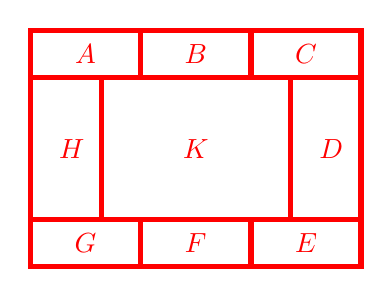
\begin{tikzpicture}[scale=.6, line width=2pt, red]
			\def\W{7}  
			\def\H{5}  
			\def\w{4}   
			\def\h{3}  
			\draw (0,0) rectangle (\W,\H); 
			\draw ({(\W-\w)/2},{(\H-\h)/2}) rectangle ({(\W+\w)/2},{(\H+\h)/2});  
			\draw (\W/3,\H) -- (\W/3,{(\H+\h)/2});
			\draw (2*\W/3,\H) -- (2*\W/3,{(\H+\h)/2});
			\draw (\W/3,0) -- (\W/3,{(\H-\h)/2});
			\draw (2*\W/3,0) -- (2*\W/3,{(\H-\h)/2});
			\draw (0,{(\H+\h)/2}) -- ({(\W-\w)/2},{(\H+\h)/2});
			\draw (0,{(\H-\h)/2}) -- ({(\W-\w)/2},{(\H-\h)/2});
			\draw (\W,{(\H+\h)/2}) -- ({(\W+\w)/2},{(\H+\h)/2});
			\draw (\W,{(\H-\h)/2}) -- ({(\W+\w)/2},{(\H-\h)/2});
			\node at (\W/6,{\H-0.5}) {$A$};
			\node at (\W/2,{\H-0.5}) {$B$};
			\node at (5*\W/6,{\H-0.5}) {$C$};			
			\node at (\W/8,{\H/2}) {$H$};
			\node at (\W/2,{\H/2}) {$K$};
			\node at (5*\W/5.5,{\H/2}) {$D$};			
			\node at (\W/6,{0.5}) {$G$};
			\node at (\W/2,{0.5}) {$F$};
			\node at (5*\W/6,{0.5}) {$E$};
		\end{tikzpicture}
	}
	\par
	\shortans[0]{1\,032}
	\loigiai{
		Ta mô hình hóa bài toán dưới dạng tô màu các đỉnh của đồ thị
		\begin{itemize}
			\item Vùng trung tâm $K$ tiếp giáp với tất cả $8$ vùng còn lại ($A$, $B$, $C$, $D$, $E$, $F$, $G$, $H$).
			\item $8$ vùng xung quanh tạo thành một chu trình khép kín $A-B-C-D-E-F-G-H-A$ (đồ thị chu trình $C_8$).
		\end{itemize}
		Quy trình tô màu được thực hiện qua $2$ bước
		\begin{itemize}
			\item \textbf{Bước 1: Tô màu vùng trung tâm $K$.} \\
			Vì $K$ kề với tất cả các vùng khác nên ta tô $K$ trước. Có $4$ cách chọn màu cho $K$.
			\item \textbf{Bước 2: Tô màu $8$ vùng xung quanh.} \\
			Sau khi tô $K$, các vùng xung quanh không được trùng màu với $K$. Do đó, ta cần tô màu cho chu trình $C_8$ gồm $8$ đỉnh bằng $3$ màu còn lại ($4$ màu ban đầu trừ đi màu của $K$).
		\end{itemize}
		Xét bài toán phụ (chứng minh công thức tô màu chu trình):\\
		Gọi $a_n$ là số cách tô màu cho chu trình $n$ đỉnh ($C_n$) bằng $\lambda$ màu sao cho $2$ đỉnh kề nhau khác màu ($n \geq 3$).
		\begin{itemize}
			\item Xét một hàng dọc $n$ đỉnh (không nối đầu đuôi).\\ Đỉnh đầu có $\lambda$ cách chọn, các đỉnh sau mỗi đỉnh có $\lambda-1$ cách chọn (khác đỉnh liền trước).\\ Tổng số cách là $\lambda(\lambda-1)^{n-1}$.
			\item Trong $\lambda(\lambda-1)^{n-1}$ cách tô hàng dọc này, có $2$ trường hợp xảy ra đối với đỉnh đầu ($1$) và đỉnh cuối ($n$)
			\begin{enumerate}
				\item Đỉnh ($1$) và đỉnh ($n$) \textbf{khác} màu: Đây chính là số cách tô màu hợp lệ cho chu trình $C_n$ (vì khi nối lại chúng thỏa mãn điều kiện kề nhau khác màu). Số cách là $a_n$.
				\item Đỉnh ($1$) và đỉnh ($n$) \textbf{cùng} màu: Khi chập đỉnh ($1$) và ($n$) lại thành $1$, ta được một chu trình nhỏ hơn là $C_{n-1}$. Số cách là $a_{n-1}$.
			\end{enumerate}
			\item Từ đó ta có hệ thức truy hồi: $a_n + a_{n-1} = \lambda(\lambda-1)^{n-1}$.
			\item Ta chứng minh công thức tổng quát là $a_n = (\lambda-1)^n + (-1)^n(\lambda-1)$ bằng quy nạp hoặc thay vào hệ thức
			\begin{align*}
				VT &= [(\lambda-1)^n + (-1)^n(\lambda-1)] + [(\lambda-1)^{n-1} + (-1)^{n-1}(\lambda-1)] \\
				&= (\lambda-1)^{n-1} [(\lambda-1) + 1] + (\lambda-1) [(-1)^n + (-1)^{n-1}] \\
				&= (\lambda-1)^{n-1} \cdot \lambda + (\lambda-1) \cdot 0 \\
				&= \lambda(\lambda-1)^{n-1} = VP \quad (\text{đúng}).
			\end{align*}
		\end{itemize}
		\textbf{Áp dụng vào bài toán:}
		tô chu trình $8$ đỉnh ($n=8$) với số màu là $3$ ($\lambda=3$):
		\[ a_8 = (3-1)^8 + (-1)^8(3-1) = 2^8 + 2 = 256 + 2 = 258 \text{ (cách)}.\]
		Theo quy tắc nhân, tổng số cách tô màu cho $9$ vùng là
		\[ 4 \cdot 258 = 1\,032 \text{ (cách)}. \]
	}
\end{ex}
%%%=============================%%%

%%%=============EX_19=============%%%
\begin{ex}%[2D1V3-6]%[TDMZD01]%[Đình Nguyên]
	Nhà máy $X$ chuyên sản xuất một loại sản phẩm cho nhà máy $Y$. Hai nhà máy thỏa thuận với nhau: Hàng tháng $X$ cung cấp cho $Y$ tối đa $150$ sản phẩm và tối thiểu $1$ sản phẩm, giá bán mỗi đơn vị sản phẩm là $p(x)=900-0{,}023x^2$ (nghìn đồng), hàng tháng $X$ chịu một chi phí cố định để sản xuất loại sản phẩm này là $750$ nghìn đồng và chi phí sản xuất mỗi sản phẩm hết $54$ nghìn đồng. Nếu coi như $X$ chỉ sản xuất theo đơn đặt hàng của $Y$ (tức là tất cả các sản phẩm sản xuất ra, thì $Y$ đều mua hết). Hãy xác định số lượng sản phẩm mà nhà máy $X$ cần sản xuất trong một tháng để thu được lợi nhuận lớn nhất.
	\par
	\shortans[0]{111}
	\loigiai{
		Gọi $x$ là số lượng sản phẩm nhà máy $X$ sản xuất trong một tháng ($1 \leq x \leq 150$, $x \in \mathbb{N}$).\\
		Doanh thu của nhà máy $X$ thu được trong một tháng là
		\[R(x) = x \cdot p(x) = x(900 - 0{,}023x^2) = 900x - 0{,}023x^3 \text{ (nghìn đồng).}\]
		Tổng chi phí nhà máy $X$ bỏ ra trong một tháng là
		\[C(x) = 54x + 750 \text{ (nghìn đồng).}\]
		Lợi nhuận nhà máy $X$ thu được là
		\allowdisplaybreaks
		\begin{eqnarray*}
			L(x) = R(x)-C(x)&=& 900x - 0{,}023x^3 - (54x + 750)\\
			&=& -0{,}023x^3 + 846x - 750.
		\end{eqnarray*}
		Xét hàm số $L(x) = -0{,}023x^3 + 846x - 750$ trên đoạn $[1; 150]$.\\
		Ta có $L'(x) = -0{,}069x^2 + 846$.\\
		Khi đó $L'(x) = 0 \Leftrightarrow -0{,}069x^2 + 846 = 0 \Leftrightarrow x^2 = \dfrac{846}{0{,}069} \Rightarrow x \approx 110{,}73$.\\
		Bảng biến thiên
		\begin{center}
			
\begin{tikzpicture}[scale=1, font=\footnotesize, line join=round, line cap=round, >=stealth]
				\tkzTabInit[nocadre=false, lgt=1.2, espcl=2.5, deltacl=0.6]
				{$x$ /0.6,$L'(x)$ /0.6,$L(x)$ /2}
				{$1$, $110{,}73$, $150$}
				\tkzTabLine{,+,0,-,}
				\tkzTabVar{-/ $95{,}977$, +/ $L(110{,}73)$, -/ $48\,675$}
			\end{tikzpicture}
		\end{center}
		Vì $x$ là số nguyên nên ta so sánh lợi nhuận tại $x=110$ và $x=111$.
		\begin{itemize}
			\item Với $x=110$: $L(110) = -0{,}023 \cdot 110^3 + 846 \cdot 110 - 750 = 61\,697$ (nghìn đồng).
			\item Với $x=111$: $L(111) = -0{,}023 \cdot 111^3 + 846 \cdot 111 - 750 = 61\,700{,}487$ (nghìn đồng).
		\end{itemize}
		Vậy nhà máy cần sản xuất $111$ sản phẩm để thu được lợi nhuận lớn nhất.
	}
\end{ex}
%%%=============================%%%

%%%=============EX_20=============%%%
\begin{ex}%[2D4V3-2]%[TDMZD01]%[Nguyễn Văn Sang]
	\immini[thm]
	{Cho một kim tự tháp mô hình là một hình chóp đều $S. ABCD$ có cạnh đáy bằng $40$ cm và cạnh bên bằng $60$ cm. Ở mỗi mặt bên người ta sơn màu cho một hình phẳng giới hạn bởi đường parabol có trục đối xứng trùng với trục đối xứng của mặt bên, tiếp xúc với hai cạnh bên tại các đỉnh của đáy. Hãy tính theo centimet vuông tổng diện tích đã được sơn màu (\textit{làm tròn kết quả đến hàng đơn vị}).
	}
	{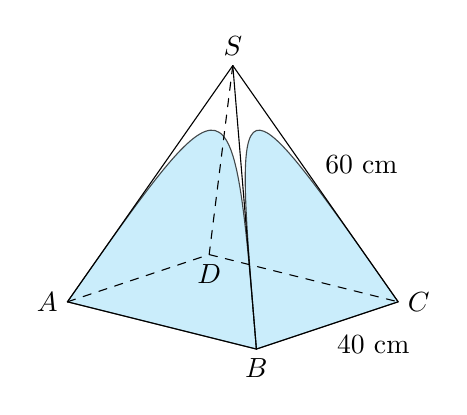
\begin{tikzpicture}[scale=0.6, line join=round, line cap=round, >=stealth]
			\coordinate (A) at (-3,-1);
			\coordinate (B) at (1,-2);
			\coordinate (C) at (4,-1);
			\coordinate (D) at (0,0);
			\coordinate (O) at (0.5,-1);
			\coordinate (S) at (0.5, 4);
			\def\parabolacolor{cyan!30}
			\draw[fill=\parabolacolor, opacity=0.7] (A) .. controls (S) .. (B) -- cycle;
			\draw[fill=\parabolacolor, opacity=0.7] (B) .. controls (S) .. (C) -- cycle;
			\draw (S)--(A) (S)--(B);
			\draw (S)--(C) node[midway, above right] {$60$ cm};
			\draw (A)--(B);
			\draw (B)--(C) node[midway, below right] {$40$ cm};
			\draw[dashed] (S)--(D) (A)--(D)--(C);
			\node[left] at (A) {$A$};
			\node[below] at (B) {$B$};
			\node[right] at (C) {$C$};
			\node[below] at (D) {$D$};
			\node[above] at (S) {$S$};
	\end{tikzpicture}}
	\par
	\shortans[0]{3\,017}
	\loigiai{
		\immini
		{ Xét mặt bên $SAB$ là tam giác cân tại $S$ với $AB = 40$ cm và\break $SA = SB = 60$ cm.\\
			Gọi $M$ là trung điểm của $AB$, ta có $SM \perp AB$.\\
			Chiều cao của mặt bên
			\[SM = \sqrt{SA^2 - AM^2} = \sqrt{60^2 - 20^2} = \sqrt{3\,200} = 40\sqrt{2} \text{ (cm)}.\]
			Chọn hệ trục tọa độ $Oxy$ gắn với mặt bên $SAB$ sao cho gốc tọa độ $O$ trùng với trung điểm $M$ của $AB$, tia $Ox$ trùng với tia $MB$, tia $Oy$ trùng với tia $MS$.\\
			Khi đó $M(0;0)$, $A(-20;0)$, $B(20;0)$, $S(0; 40\sqrt{2})$.\\
			Gọi phương trình parabol $(P)$ là $y = ax^2 + bx + c$.}
		{\begin{tikzpicture}[scale=0.6, line join=round, line cap=round, >=stealth]
				\coordinate (A) at (-3,-1);
				\coordinate (B) at (1,-2);
				\coordinate (C) at (4,-1);
				\coordinate (D) at (0,0);
				\coordinate (O) at (0.5,-1);
				\coordinate (S) at (0.5, 4);
				\def\parabolacolor{cyan!30}
				\draw[fill=\parabolacolor, opacity=0.7] (A) .. controls (S) .. (B) -- cycle;
				\draw[fill=\parabolacolor, opacity=0.7] (B) .. controls (S) .. (C) -- cycle;
				\coordinate (M) at ($(A)!0.5!(B)$);
				\draw (S)--(M);
				\fill (M) circle (1.5pt) node[below] {$M$};
				\draw (S)--(A) (S)--(B) (S)--(C);
				\draw (A)--(B)--(C);
				\draw[dashed] (S)--(D) (A)--(D)--(C);
				\node[left] at (A) {$A$};
				\node[below] at (B) {$B$};
				\node[right] at (C) {$C$};
				\node[below] at (D) {$D$};
				\node[above] at (S) {$S$};
		\end{tikzpicture}}
		\noindent
		Vì trục đối xứng của parabol trùng với $SM$ (trục $Oy$) nên $b = 0$.\\ Suy ra $(P)\colon y = ax^2 + c$.\\
		Parabol đi qua $A(-20;0)$ nên $0 = 400a + c \Rightarrow c = -400a$\quad($\ast$).\\
		Đường thẳng chứa cạnh bên $SA$ đi qua $A(-20;0)$ và $S(0; 40\sqrt{2})$ có hệ số góc
		\[k = \dfrac{40\sqrt{2} - 0}{0 - (-20)} = 2\sqrt{2}.\]
		Vì parabol tiếp xúc với cạnh bên $SA$ tại $A$ nên đạo hàm tại $x_A = -20$ bằng hệ số góc $k$.\\
		Ta có $y' = 2ax$.\\
		Tại $x = -20 \Rightarrow y'(-20) = -40a$.\\
		Suy ra $-40a = 2\sqrt{2} \Rightarrow a = -\dfrac{\sqrt{2}}{20}$.\\
		Thay vào ($\ast$) ta được $c = -400 \cdot \left(-\dfrac{\sqrt{2}}{20}\right) = 20\sqrt{2}$.\\
		Vậy phương trình parabol là $y = -\dfrac{\sqrt{2}}{20}x^2 + 20\sqrt{2}$.\\
		Diện tích phần được sơn trên một mặt bên là diện tích giới hạn bởi parabol và trục hoành (cạnh đáy $AB$)
		\allowdisplaybreaks
		\begin{eqnarray*}
			S_1
			&=& \displaystyle\int\limits_{-20}^{20} \left(-\dfrac{\sqrt{2}}{20}x^2 + 20\sqrt{2}\right) \,\mathrm{d}x \\
			&=& \left[ -\dfrac{\sqrt{2}}{60}x^3 + 20\sqrt{2}x \right]\Bigg|_{-20}^{20} \\
			&=& \left( -\dfrac{\sqrt{2}}{60} \cdot 8\,000 + 400\sqrt{2} \right) - \left[-\dfrac{\sqrt{2}}{60} \cdot (-8\,000) + (-400)\sqrt{2} \right]\\
			&=& \dfrac{800\sqrt{2}}{3} \left(\mathrm{cm}^2\right).
		\end{eqnarray*}
		Tổng diện tích được sơn trên $4$ mặt bên là
		\[S = 4 S_1 = 4 \cdot \dfrac{800\sqrt{2}}{3} = \dfrac{3\,200\sqrt{2}}{3} \approx 3\,016{,}98.\]
		Làm tròn đến hàng đơn vị, ta được $S \approx 3\,017$\,(cm$^2$).
	}
\end{ex}
%%%=============================%%%

%%%=============EX_21=============%%%
\begin{ex}%[2H2V2-6]%[TDMZD01]%[Đoàn Văn Mùi]
	\immini[thm]{ Trong không gian $Oxyz$ (đơn vị trên mỗi trục là mét), một tấm tròn được mô hình hoá nằm trên mặt phẳng toạ độ $(Oxy)$, có tâm $O$ và bán kính $r=4$. Ở cùng một thời điểm có vật $M$ bắt đầu chuyển động từ điểm
		$A(2;-8;-2)$ với vectơ vận tốc $\overrightarrow{u}=(0;1;0)$ và vật $N$ bắt đầu chuyển động từ điểm $B(12;0;2)$ với vectơ vận tốc $\overrightarrow{v}=(-1;0;0)$. Biết đơn vị của các vận tốc là m/s. Hãy xác định theo giây khoảng thời gian mà vật $M$ không nhìn được vật $N$ \textit{(làm tròn kết quả đến hàng phần mười)}.}{
		\begin{tikzpicture}[declare function={r=3;}]
			\path (0,0) coordinate (O)
			(-2,-1.5)  coordinate (A)
			(4,-1.5)  coordinate (A')
			($(A)+(0,.2)$) coordinate (x)
			($(x)+(1,0)$) coordinate (y)
			($(A)+(0,2)$) coordinate (B)
			($(A')+(0,4)$) coordinate (B')
			($(B)+(0,.2)$) coordinate (x')
			($(B)!.2!(B')$) coordinate (t)
			($(x')+(t)-(B)$) coordinate (y')
			;
			
			\fill[blue,opacity=0.3] (O) ellipse (1cm and .5cm);
			\draw[dashed] (A)--(A') (B)--(B');
			\draw (O) ellipse (1cm and .5cm);
			\draw[->] (x)--(y);
			\draw[->] (x')--(y');
			\node at (1.5,1) {$(C)$};
			\foreach \t/\g in {A/180,B/180}{
				\draw[fill=black] (\t) circle (1pt) node[shift={(\g:7pt)},font=\scriptsize]{$ \t $};
			}
		\end{tikzpicture}
	}
	\par
	\shortans[0]{9,6}
	\loigiai{
		Tọa độ $M_t(2; -8+t; -2)$, $N_t(12-t; 0; 2)$.\\
		$M$ không nhìn thấy $N$ khi đoạn $MN$ cắt tấm tròn ($x^2+y^2 \leq 16$, $z=0$).\\
		Giao điểm $I$ của $MN$ với mặt phẳng $z=0$ là trung điểm $MN$ (do $z_M=-2$, $z_N=2$).\\ Suy ra $I_t\left( \dfrac{14-t}{2}; \dfrac{t-8}{2}; 0 \right)$.\\
		Điều kiện bị chắn
		\allowdisplaybreaks
		\begin{eqnarray*}
			&&x_I^2 + y_I^2 \leq 16
			\\
			&\Leftrightarrow&\left(\frac{14-t}{2}\right)^2 + \left(\frac{t-8}{2}\right)^2 \leq 16
			\\
			&\Leftrightarrow& (t-14)^2 + (t-8)^2 \leq 64
			\\
			&\Leftrightarrow&2t^2 - 44t + 196 \leq 0
			\\
			&\Leftrightarrow& t^2 - 22t + 98 \leq 0
			\\
			&\Leftrightarrow& 11-\sqrt{23} \leq t \leq 11+\sqrt{23}.
		\end{eqnarray*}
		Khoảng thời gian $\Delta t = \left(11+\sqrt{23}\right) - \left(11-\sqrt{23}\right) = 2\sqrt{23} \approx 9{,}59$ (giây).
	}
\end{ex}
%%%=============================%%%

%%%=============EX_22=============%%%
\begin{ex}%[2D6V2-4]%[TDMZD01]%[Nguyễn Trí Minh Tuấn]
	Lớp $12A$ có $x$ học sinh nam và $15$ học sinh nữ, lớp $12B$ có $25$ học sinh nam và $10$ học sinh nữ.
	Chọn ngẫu nhiên ba em học sinh từ lớp $12A$ và hai học sinh từ lớp $12B$ để lập thành một tổ năm em học sinh đi dự đại hội chi đoàn.
	Chọn ngẫu nhiên một trong năm em học sinh này bầu làm tổ trưởng.
	Biết xác suất học sinh lớp $12A$ được làm tổ trưởng, nếu biết học sinh nữ được làm tổ trưởng, không bé hơn $0{,}6$. Hãy tìm giá trị lớn nhất của $x$.
	\par
	\shortans[0]{37}
	\loigiai{
		\textbf{\underline{CÁCH 1}}\\
		\noindent
		Gọi $A$ là biến cố \lq\lq tổ trưởng thuộc lớp $12A$\rq\rq \, và $B$ là biến cố \lq\lq tổ trưởng là nữ\rq\rq.\\
		Với cách chọn $3$ HS từ $12A$, chọn $2$ HS từ $12B$, rồi chọn $1$ tổ trưởng trong $5$ HS.
		Ta có
		\[
		n\left(\Omega\right)=\mathrm{C}_{x+15}^{3}\cdot \mathrm{C}_{35}^{2}\cdot 5.
		\]
		Để tổ trưởng vừa là nữ vừa thuộc $12A$
		\begin{itemize}
			\item Chọn tổ trưởng là một nữ của $12A$ có $\mathrm{C}_{15}^{1}$ cách;
			\item Chọn thêm $2$ HS còn lại của $12A$ từ $x+14$ HS còn lại có $\mathrm{C}_{x+14}^{2}$ cách;
			\item Chọn $2$ HS của $12B$ có $\mathrm{C}_{35}^{2}$ cách.
		\end{itemize}
		Vậy số cách chọn để tổ trưởng vừa là nữ vừa thuộc $12A$ là
		\[
		n\left(A\cap B\right)=\mathrm{C}_{15}^{1}\mathrm{C}_{x+14}^{2}\mathrm{C}_{35}^{2}.
		\]
		Để tổ trưởng là nữ, ta có
		\begin{itemize}
			\item Tổ trưởng là nữ thuộc $12A$ có $n\left(A\cap B\right)=\mathrm{C}_{15}^{1}\mathrm{C}_{x+14}^{2}\mathrm{C}_{35}^{2}$ cách.
			\item Tổ trưởng là nữ thuộc $12B$
			\begin{itemize}
				\item Chọn tổ trưởng trong $10$ nữ của $12B$ có $\mathrm{C}_{10}^{1}$ cách;
				\item Chọn thêm $1$ HS còn lại của $12B$ từ $34$ HS còn lại có $\mathrm{C}_{34}^{1}$ cách;
				\item Chọn $3$ HS của $12A$ có $\mathrm{C}_{x+15}^{3}$ cách.
			\end{itemize}
			Do đó số cách là $\mathrm{C}_{10}^{1}\mathrm{C}_{34}^{1}\mathrm{C}_{x+15}^{3}$.
		\end{itemize}
		Suy ra
		\[
		n\left(B\right)=\mathrm{C}_{15}^{1}\mathrm{C}_{x+14}^{2}\mathrm{C}_{35}^{2}+\mathrm{C}_{10}^{1}\mathrm{C}_{34}^{1}\mathrm{C}_{x+15}^{3}.
		\]
		Do đó
		\[
		\mathrm{P}\left(A\mid B\right)=\dfrac{n\left(A\cap B\right)}{n\left(B\right)}
		=\dfrac{\mathrm{C}_{15}^{1}\mathrm{C}_{x+14}^{2}\mathrm{C}_{35}^{2}}
		{\mathrm{C}_{15}^{1}\mathrm{C}_{x+14}^{2}\mathrm {C}_{35}^{2}+\mathrm{C}_{10}^{1}\mathrm {C}_{34}^{1}\mathrm{C}_{x+15}^{3}}
		\geq \dfrac{3}{5}.
		\]
		Ta có
		\[
		\mathrm{C}_{x+14}^{2}=\dfrac{(x+14)(x+13)}{2},\qquad
		\mathrm{C}_{x+15}^{3}=\dfrac{(x+15)(x+14)(x+13)}{6}.
		\]
		Bất phương trình, trở thành
		\begin{align*}
			&\dfrac{15\cdot \dfrac12\cdot \mathrm{C}_{35}^{2}}
			{15\cdot \dfrac12\cdot \mathrm{C}_{35}^{2}+10\cdot 34\cdot \dfrac{x+15}{6}}
			\geq \dfrac35 \\[6pt]
			\Leftrightarrow\;&
			\dfrac{\dfrac{8\,925}{2}}
			{\dfrac{8\,925}{2}+\dfrac{170}{3}(x+15)}
			\geq \dfrac35 \\[6pt]
			\Leftrightarrow\;&
			5\cdot \dfrac{8\,925}{2}
			\geq 3\left(\dfrac{8\,925}{2}+\dfrac{170}{3}(x+15)\right) \\[6pt]
			\Leftrightarrow\;&
			8\,925 \geq 170(x+15) \\[6pt]
			\Leftrightarrow\;&
			x \leq 37{,}5.
		\end{align*}
		Vậy giá trị lớn nhất của $x$ là $37$.\\
		\textbf{\underline{CÁCH 2}}\\
		\noindent
		Gọi $A$ là biến cố \lq\lq tổ trưởng thuộc lớp $12A$\rq\rq \, và $B$ là biến cố \lq\lq tổ trưởng là nữ\rq\rq.\\
		Khi đó $\overline{A}$ là biến cố \lq\lq tổ trưởng thuộc lớp $12B$\rq\rq \, và $\overline{B}$ là biến cố \lq\lq tổ trưởng không là nữ\rq\rq.\\
		Ta có sơ đồ cây như sau
		\begin{center}
			\begin{tikzpicture}[node distance=2.2cm, every node/.style={fill=none}, align=center,scale=0.6,font=\footnotesize]
				\definecolor{diagram_bg_green}{HTML}{d5e8d4}
				\definecolor{diagram_bg_blue}{HTML}{dae8fc}
				\definecolor{diagram_bg_pink}{HTML}{f8cecc}
				\definecolor{diagram_bd_green}{HTML}{82b366}
				\definecolor{diagram_bd_blue}{HTML}{7494c2}
				\definecolor{diagram_bd_pink}{HTML}{b85450}
				\tikzset{
					>={Latex[width=2mm,length=2mm]},
					base/.style = {rectangle, rounded corners, draw=black, minimum width=1cm, text centered,
						drop shadow={shadow xshift=0.6mm, shadow yshift=-0.6mm}},
					Style1/.style = {base, fill=diagram_bg_blue, draw=diagram_bd_blue},
					Style2/.style = {base, fill=diagram_bg_pink, draw=diagram_bd_pink},
					Style3/.style = {base, fill=diagram_bg_green, draw=diagram_bd_green},
					Style4/.style = {base, minimum width=2.5cm, fill=orange!15, draw=orange},
				}
				
				\node (B0)  [Style1, text width=1cm] {Tổ trưởng};
				
				\node (B1)  [Style2, right of=B0, xshift=3cm, yshift=1.6cm, text width=3cm] {Tổ trưởng thuộc lớp $12A$};
				\node (B3)  [Style2, right of=B0, xshift=3cm, yshift=-1.6cm, text width=3cm] {Tổ trưởng thuộc lớp $12B$};
				
				\node (B11) [Style3, right of=B1, xshift=6cm, yshift=0.9cm,  text width=4cm] {Nữ tổ trưởng};
				\node (B13) [Style3, right of=B1, xshift=6cm, yshift=-0.9cm, text width=4cm] {Nữ không tổ trưởng};
				
				\node (B31) [Style3, right of=B3, xshift=6cm, yshift=0.9cm,  text width=4cm] {Nữ tổ trưởng};
				\node (B33) [Style3, right of=B3, xshift=6cm, yshift=-0.9cm, text width=4cm] {Nữ không tổ trưởng};
				
				\draw[->] (B0) -- (B1.west) node[sloped,above,pos=0.5] {$\mathrm{P}(A)=\dfrac{3}{5}$};
				\draw[->] (B0) -- (B3.west) node[sloped,below,pos=0.5] {$\mathrm{P}\left(\overline{A}\right)=\dfrac{2}{5}$};
				
				\draw[->] (B1) -- (B11.west) node[sloped,above,pos=0.5] {$\mathrm{P}\left(B\mid A\right)=\dfrac{15}{x+15}$};
				\draw[->] (B1) -- (B13.west) node[sloped,below,pos=0.5] {$\mathrm{P}\left(\overline{B}\mid A\right)=\dfrac{x}{x+15}$};
				
				\draw[->] (B3) -- (B31.west) node[sloped,above,pos=0.5] {$\mathrm{P}\left(B\mid\overline{A}\right)=\dfrac{10}{35}$};
				\draw[->] (B3) -- (B33.west) node[sloped,below,pos=0.5] {$\mathrm{P}\left(\overline{B}\mid\overline{A}\right)=\dfrac{25}{35}$};
			\end{tikzpicture}
		\end{center}
		Ta có $\mathrm{P}\left(AB\right)=\mathrm{P}(A)\cdot\mathrm{P}\left(B\mid A\right)=\dfrac{3}{5}\cdot\dfrac{15}{x+15}=\dfrac{9}{x+15}$;\\[4pt]
		$\mathrm{P}\left(B\right)=\mathrm{P}(A)\cdot\mathrm{P}\left(B\mid A\right)+\mathrm{P}\left(\overline{A}\right)\cdot\mathrm{P}\left(B\mid \overline{A}\right)=\dfrac{9}{x+15}+\dfrac{4}{35}$.\\
		Do xác suất học sinh lớp $12A$ được làm tổ trưởng, nếu biết học sinh nữ được làm tổ trưởng, không bé hơn $0{,}6$ nên ta có
		\[
		\mathrm{P}\left(A\mid B\right)=\dfrac{\mathrm{P}\left(AB\right)}{\mathrm{P}\left(B\right)}
		=\dfrac{\dfrac{9}{x+15}}{\dfrac{9}{x+15}+\dfrac{4}{35}}
		\geq \dfrac{3}{5}.
		\]
		Suy ra $x\leq 37{,}5$. \\
		Vậy giá trị lớn nhất của $x$ là $37$.
	}
\end{ex}
%%%=============================%%%
\Closesolutionfile{ans}

\newpage
\indapan{12}{ans/ansTN-Dung}
\indapan[TF]{2}{ans/ansTN-DungSai}
\indapan[SA]{4}{ans/ansTN-DienKhuyet}
%%%%%%%%%%%%%%
%%nhãn kết thúc đề (để đếm số trang tự động mỗi đề)
\label{B\thedeso}